%RLC_Circuits_P2
\chapter{AC Voltages and the Arduino}

\objectives
{
\item Use an Arduino to measure AC voltages.
\item Describe the problem of ``aliasing'', and how it can be mitigated.
}

In the second lab of the semester, we learned how to use an oscilloscope to
measure AC voltages. We would like to be able to do this with the Arduino as
well. 
Some complications arise, however, when we try to use an Arduino as an 
oscilloscope:
\begin{itemize}
	\item The Arduino can only handle input voltages up to 5 Volts
		(we've already learned how to mitigate this issue via the
		use of a voltage divider).
	\item The Arduino cannot handle negative voltages (which can - and
		probably will - destroy the Arduino).
	\item The Arduino may not be able to sample voltages fast enough.
\end{itemize}
In this lab, we will see how we can get around these issues.

\section{The Instrument}

The first challenge we face is that the voltage from the RLC circuit is
sometimes negative (see Figure \ref{fig:rlc_signal}).
We will have truly negative voltages compared to our ground. Can
we send a negative voltage into our Arduino? The answer is an emphatic NO!
Negative voltages will destroy our Arduino, just as easily as high
voltages. But we really have a
sinusoidal signal. 
\begin{figure}[htbp!]
\centering
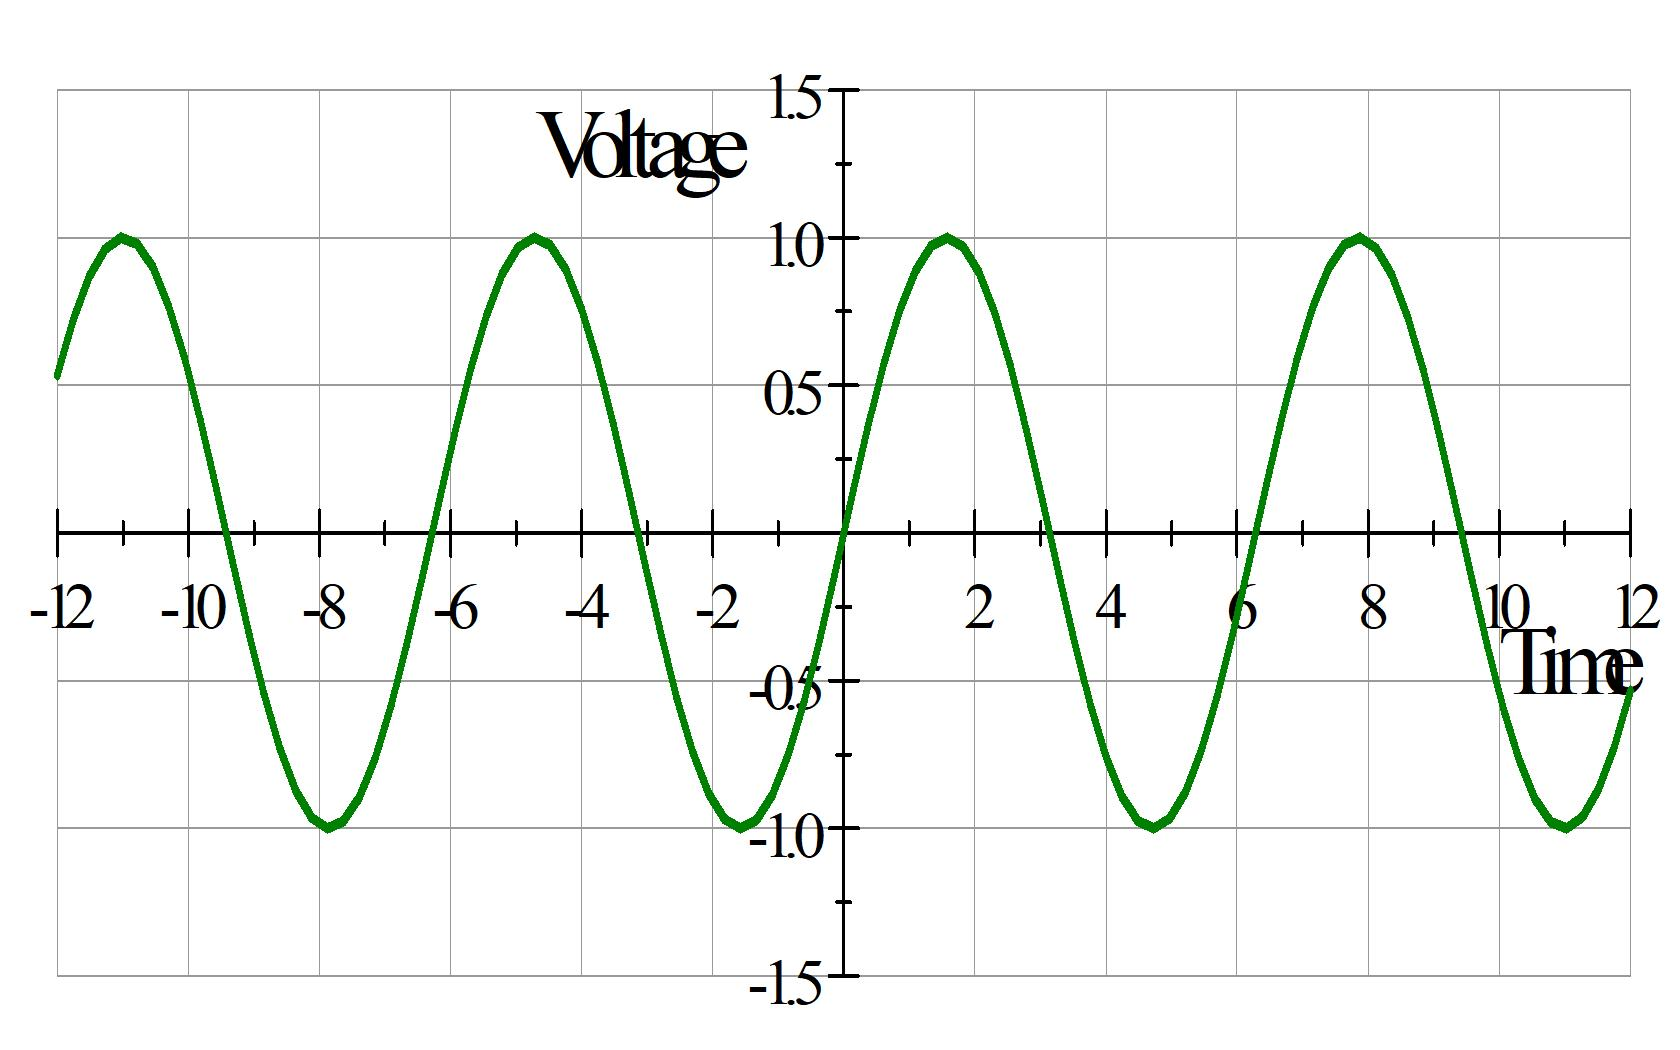
\includegraphics[width=\textwidth]{PH4CAX4H}
	\caption{The AC signal coming from an RLC circuit.}
	\label{fig:rlc_signal}
\end{figure}

The easiest way to fix this problem is, once again, to use a voltage
divider - only this time we will fix each end at a different voltage. We will
need one end at a positive voltage. The other can then go as negative as the
first end is positive. Let's take a concrete example to show how this works.

Suppose we want to measure a voltage that could be as negative as $-5\unit{V}
$ or as positive as $+5\unit{V}.$ We still need to map this to our $0$ to $5%
\unit{V}$ Arduino range. Consider the voltage divider seen in Figure
\ref{fig:rlc_vd}.
Let's start by setting $R_{1}=R_{2}.$ Then, any voltage at the junction
between $R_{1}$ and $R_{2}$ should be midway between the voltages input on
the top of $R_{1}$ and the Bottom of $R_{2}.$ We put in $+5\unit{V}$ from
our power supply on the top. And suppose we hook $-5\unit{V}$ to the bottom
(say, from our signal generator). We expect the voltage divider to divide
the total voltage difference in half. We have $10\unit{V}$ range from $-5%
\unit{V}$ to $+5\unit{V}$. We expect the junction between $R_{1}$ and $R_{2}$
to be right in the middle of that range. So we expect to see $0\unit{V}$ on
pin A0 when the signal generator outputs $-5\unit{V}.$ So far so good! Now
suppose the signal generator gives us $+5\unit{V}.$ Half way between $+5%
\unit{V}$ and $+5\unit{V}$ is still $+5\unit{V}$. This is just what we want!
Any voltage from the signal generator between $+5\unit{V}$ and $-5\unit{V}$
will end up between $0\unit{V}$ and $+5\unit{V}$ at input A0. For example,
say we have $-2\unit{V}$ from the signal generator. The at $A0$ we will have
a voltage half way between $+5\unit{V}$ and $-2\unit{V}.$ Pin A0 would have $%
1.5\unit{V}.$
\begin{figure}[tbp!]
\centering
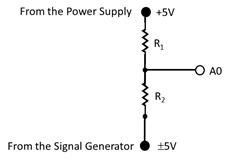
\includegraphics[width=0.5\textwidth]{PH4CAX4I}
	\caption{Using a voltage divider to positive bias a signal.}
	\label{fig:rlc_vd}
\end{figure}


We must be very careful to get this
voltage divider wired correctly before we hook it to our
Arduino. We also need to make sure our signal generator and power supply are
plugged into grounded outlets, or otherwise share a common ground. 
\emph{It is always a good idea to test the voltages at the midpoint of the
voltage divider with an
oscilloscope, prior to attaching it to pin A0 on the Arduino!}

The oscilloscope, power supply, and signal generator are all grounded
through their grounded plugs, but our Arduino is not. We need to tie all the
grounds of all our equipment together. The way to do this is to 
put a wire on the power supply
negative output and wire it with an alligator clip to the grounded exterior
of the signal generator TTL BNC connector. Then take another wire and
connect it to the power supply negative output and wire this to a GND pin
on the Arduino. This should ensure that all three devices have the same
ground point (so we won't get a spark from one to another).

Before we hook this bit of electronics to our Arduino, we want to check it
using an oscilloscope.
Our oscilloscopes have two channels where we can hook probes. Let's use one
to measure the signal as it comes directly from the signal generator. Let's
use the other to measure at the junction in between $R_{1}$ and $R_{2}$
right were we will connect pin A0. That should be our output. 
%A picture of 
%these connections can be seen in Figure \ref{fig:rlc_ground}, and a 
A schematic of the entire circuit, with the voltage divider attached,
can be seen in Figure \ref{fig:rlc_schematic}.

%\begin{figure}[htbp!]
%	\centering
%	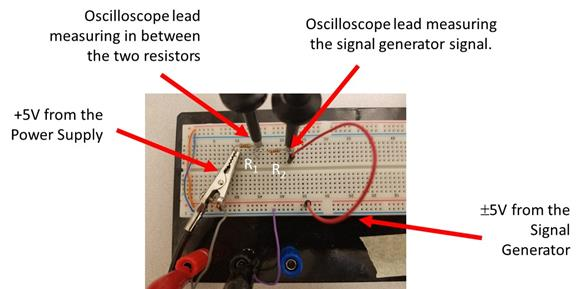
\includegraphics[width=\textwidth]{PH4CAX4J}
%	\caption{Photograph of the ground connections for the voltage 
%	divider.}
%	\label{fig:rlc_ground}
%\end{figure}
\begin{figure}[htbp!]
	\centering
	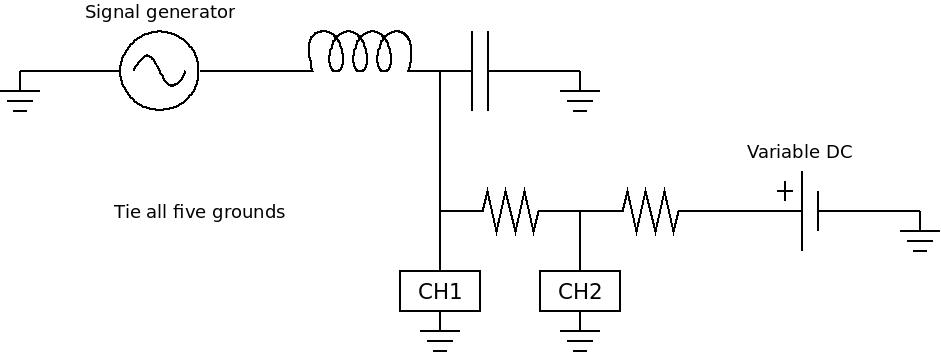
\includegraphics[width=\textwidth]{RLCschem}
	\caption[Schematic diagram of the circuit, with the
	voltage divider attached]{Schematic diagram of the 
	circuit, with the 
	voltage divider attached, grounds properly connected, and the
	oscilloscope in place.}
	\label{fig:rlc_schematic}
\end{figure}

When the circuit is built and functioning, the signals on the oscilloscope
should appear as in Figure \ref{fig:rlc_osc}.
The red trace is the voltage at the signal generator.
The yellow trace is the voltage from the midpoint of the voltage divider. 
Notice that in this figure the capacitor voltage alternates between
-5 V and +5 V, while the output from the voltage divider is from 0 to +5 V,
as desired. The yellow trace can be raised or lowered by changing the voltage
output from the DC power source.
\begin{figure}[htbp!]
	\centering
	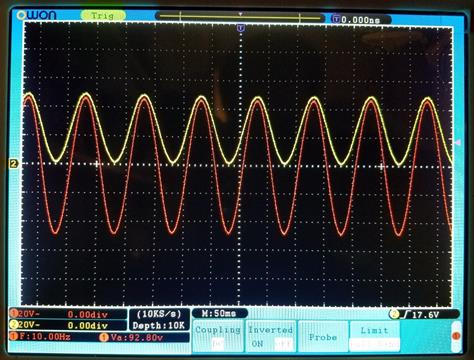
\includegraphics[width=\textwidth]{PH4CAX4K}
	\caption{Oscilliscope signal for the capacitor voltage and output
	signal from the voltage divider.}
	\label{fig:rlc_osc}
\end{figure}

Of course in our sketch, we have to do a little math to convert our 
output signal of 0 V to +5 V back into the the capacitor voltage of
-5 V to +5 V. Basically, we just have to undo our mapping. We multiply our
ADC units by two, and then subtract 5 V.
\begin{equation}
\Delta V_{measured}=2\Delta V_{ADC}-5\unit{V}
\end{equation}
Notice that our minimum detectable voltage difference of $\Delta V_{ADC\min
}=4.9\unit{mV}$ will map to 
\begin{eqnarray*}
\delta V &=&2\left( 4.9\unit{mV}\right) \\
&=&9\,.8\unit{mV}
\end{eqnarray*}
so that the minimum uncertainty in our voltage readings will be 9.8 mV.
This higher uncertainty is the price we pay for being able to measure both
positive and negative voltages.

Once again, make sure that you use the oscilloscope to measure the output
voltage from the voltage divider prior to attaching the Arduino.
We can set up our circuit and clip the oscilloscope probe to either side of
the capacitor, as seen in Figure \ref{fig:rlc_schematic}. 
%As we change the frequency of the signal generator the
%frequency of the voltage across the capacitor will change. As we get near
%the resonant frequency, the amplitude of the capacitor voltage will grow.
%Right at the resonant frequency, $\Delta V_{C}$ will be largest. We will
%need to measure this with the oscilloscope 
%before using our Arduino, just to be sure the voltage won't
%go over $5\unit{V}$. This means we need to keep the capacitor voltage
%below $\pm$5 V at resonance.
%If we keep changing the frequency the amplitude will go back
%down. So when we see the amplitude grow, max out, and then diminish we know
%we have just passed resonance. This is just what we saw in last week's lab.

Once we have this working on our oscilloscope, we can try it on our Arduino.
Of course we need a sketch for this. Here is a simple example.
\lstinputlisting[language=Arduino]{Code/RLCPart2_pm5Vsignal.ino}

%Our new instrument takes in an alternating voltage, and displays it. We
%will have to adjust the input voltage on the signal generator. When the
%signal generator frequency is just right, the voltage we measure should
%become large. By noting the resonant frequency we can check our model for
%inductance.

\section{Sampling Theory, a complication}

Before we finish, we need to think about another
limitation of our Arduino devices, which is that they can only take up to $%
2000$ measurements in a second. We say they have a maximum sampling rate of $%
2000\unit{Hz}.$ To try to understand this, consider trying to measure a sine
wave with a frequency of 1000 Hz, as seen in Figure \ref{fig:sine}.
The sine wave has a value for every one of the infinietly many possible times
depicted in the graph. That is, 
\begin{equation*}
V\left( t\right) =\sin \left( \omega t\right)
\end{equation*}%
has a defined value for every $t$ at all. In an ideal situation, if we were 
measuring this sine wave, we could measure the voltage at an infinite 
number of times between 
$0$ and $1\unit{s}$ so that we would not miss any $V\left(
t\right) $ values. 
\begin{figure}[htbp!]
	\centering
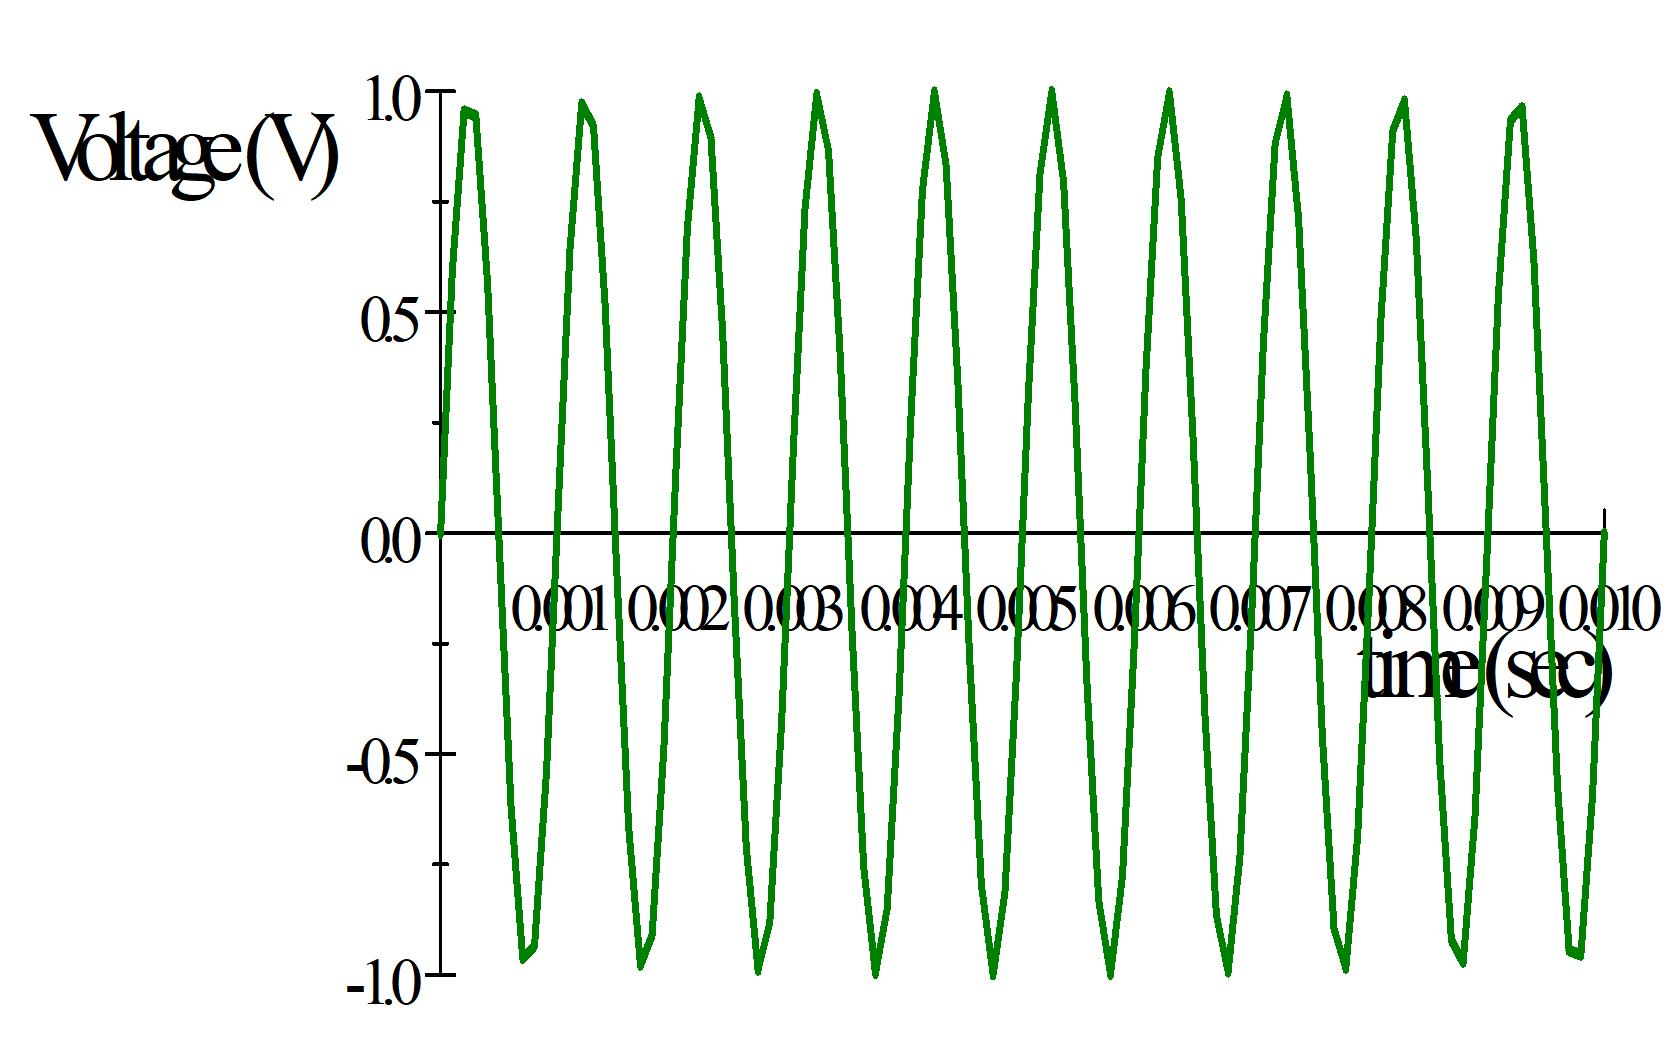
\includegraphics[width=4.4996in,height=1.7919in]{PH4CAX4L}
	\caption{A 1000 Hz sine wave.}
	\label{fig:sine}
\end{figure}

In reality, the Arduino can't take an infinite number of values.
It an only take up to $2000$ values a second, or two values for every cycle of
our sine wave. What we see in our measurement suddenly becomes very sensitive 
to where the measurements begin! If my first measurement occurred at the 
first peak in Figure \ref{fig:sine}, the next measurement would occur at
the first trough, and I would be getting an accurate view of how much the 
voltage fluctuated. However, consider what happens if that first measurement
does not occur at the first peak, as in Figure \ref{fig:sine2}. In this image,
the red dots correspond to the measurements we take. The red dots are all we
would see, and the green line represents what is actually happening. From
our measurements, we would see that the signal is oscillating, and we would
probably even deduce the right oscillation frequency. However, what we would
perceive as the maximum voltage would be very wrong!
\begin{figure}[htbp!]
	\centering
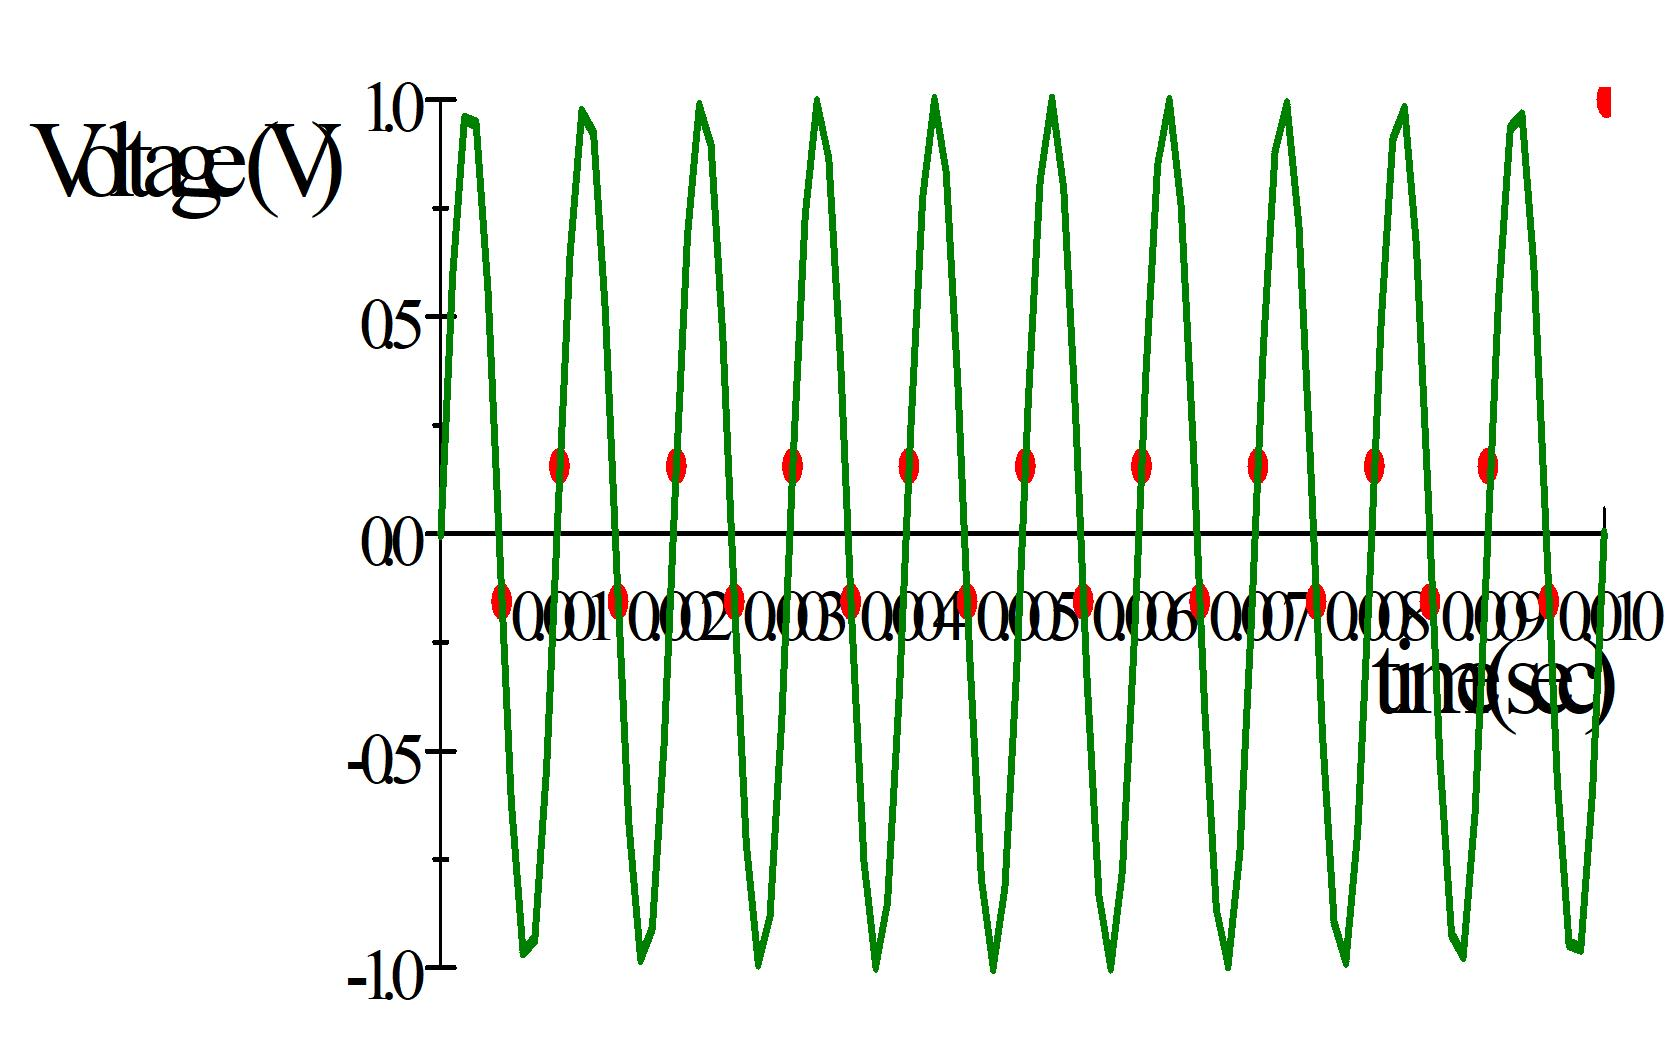
\includegraphics[width=4.4996in,height=1.6354in]{PH4CAX4N}
	\caption[Measuring a 1000 Hz signal with a 2000 Hz sampling rate]
	{Measuring a 1000 Hz signal with a 2000 Hz sampling rate, where the
	samples do not occur at the true extrema of the sine wave.}
	\label{fig:sine2}
\end{figure}

The situation can get even worse. Suppose our first sample happened to 
occur at time $t=0$. This measurement, as well as all subsequent measurements,
would fall on the nodes of the sine wave, as seen in Figure
\ref{fig:sine3}. \emph{We would only get measurements
of zero voltage!} Consequently, we would believe we were measuring a constant
zero voltage.
\begin{figure}[htbp!]
	\centering
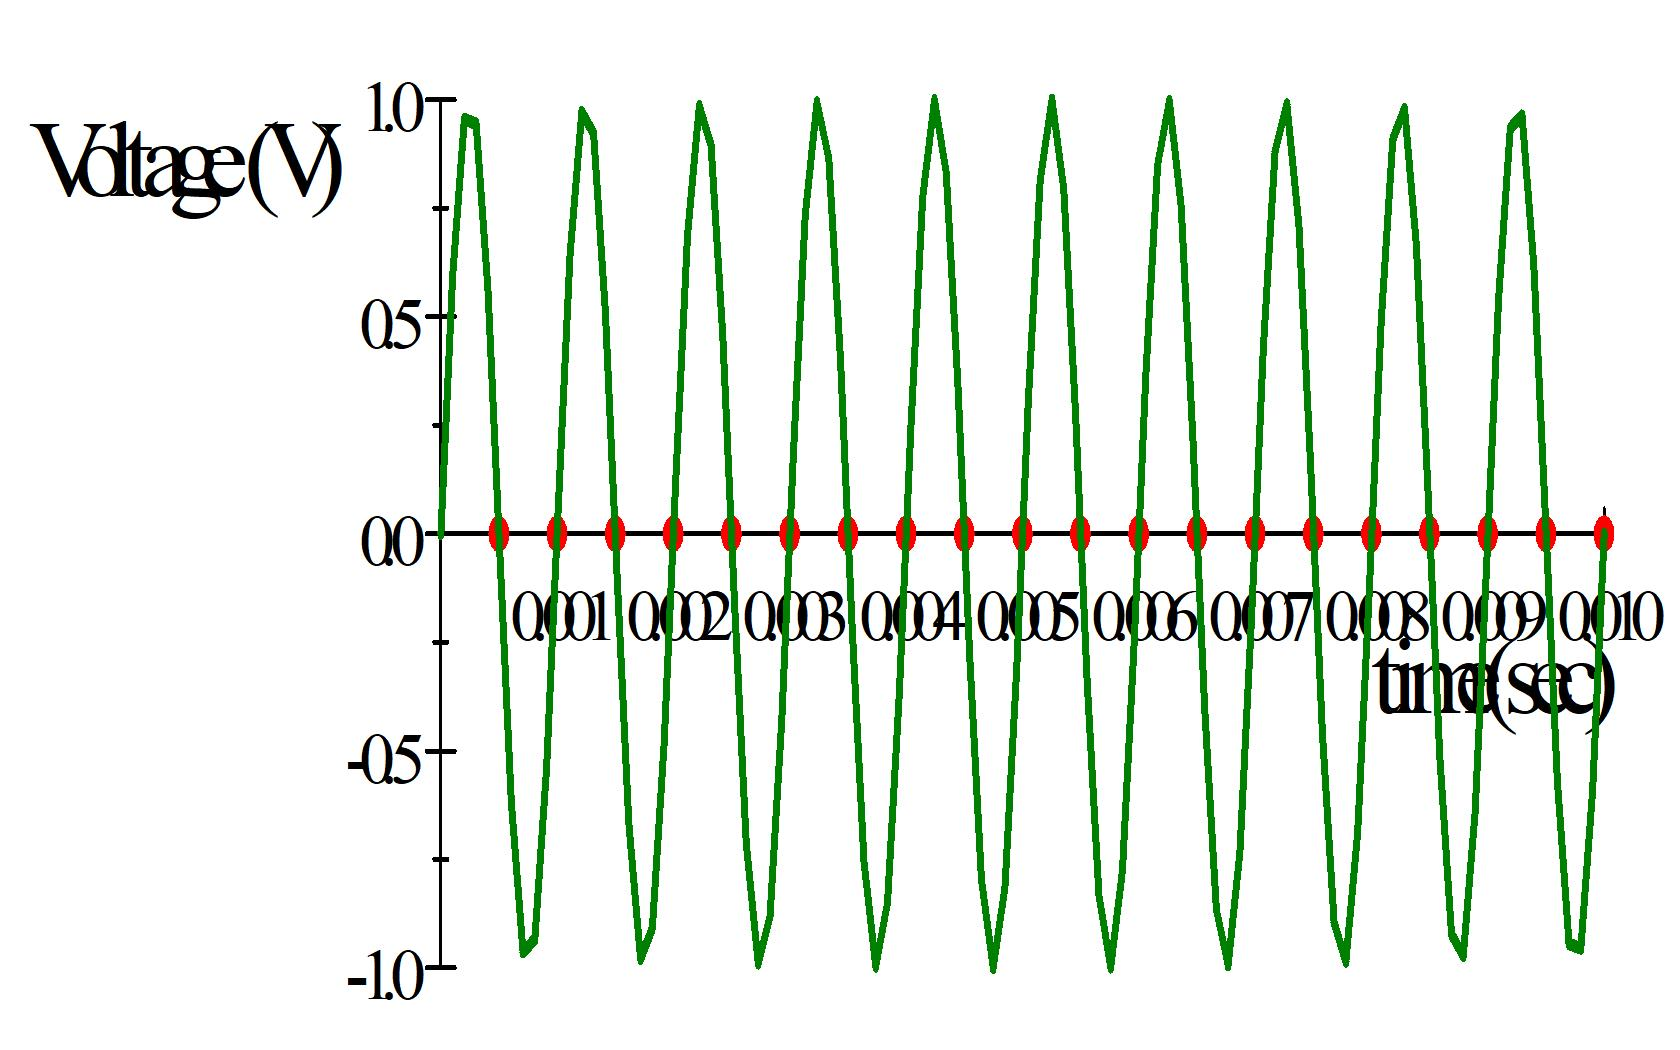
\includegraphics[width=4.4996in,height=1.6354in]{PH4CAX4M}
	\caption[Another measurement of a 1000 Hz signal with a 2000 Hz 
	sampling rate]{Another measurement of a 1000 Hz signal with a 2000 Hz
        sampling rate. In this case, all of the measured voltages would be
	zero.}
	\label{fig:sine3}
\end{figure}

The solution to this problem is to lower our signal frequency so
that we have more points per signal period. Say, we have a sine wave with a
frequency of $250\unit{Hz}$, but still with a sampling rate of 2000 Hz. This
will give us eight samples per period, and our measurements would look more 
like Figure \ref{fig:sine4}. With more samples per period, it is easier to see
the character of the sine wave. Even if our measurements were offset just 
a little in time, we would still be able to distinguish both the frequency 
and amplitude of this wave.
\begin{figure}[htbp!]
	\centering
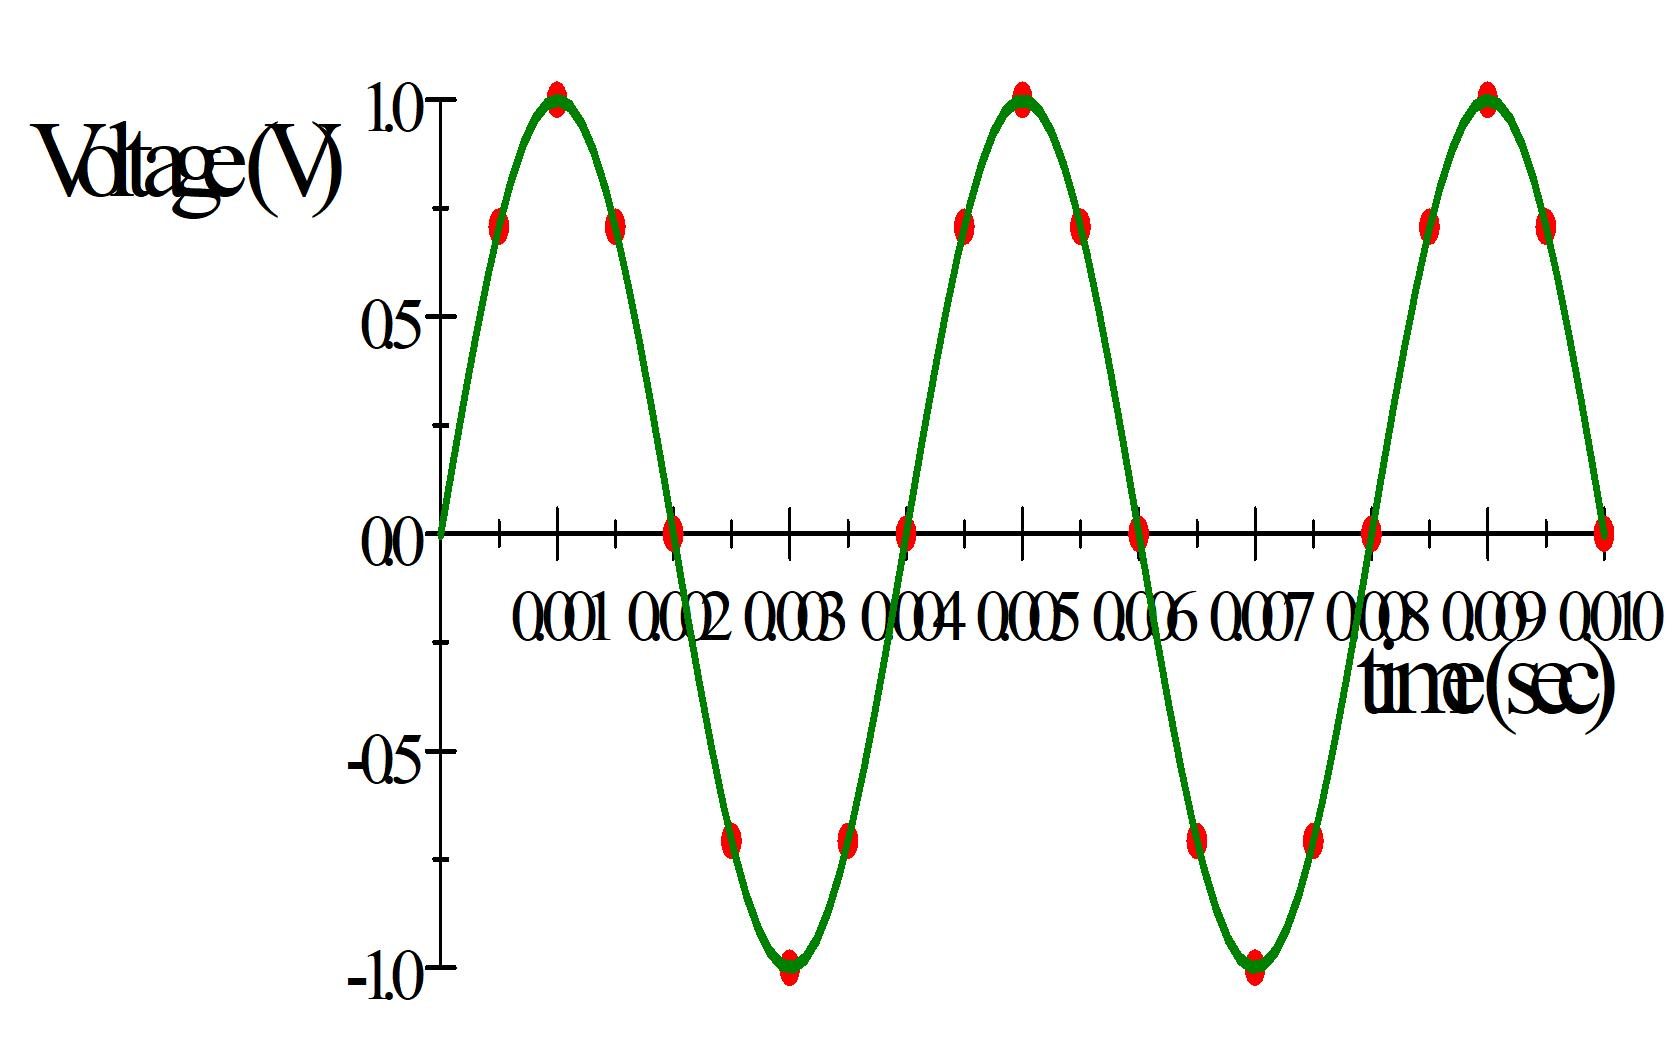
\includegraphics[width=4.4996in,height=1.6354in]{PH4CAX4O}
	\caption{Measuring a 250 Hz signal with a 2000 Hz sampling rate.}
	\label{fig:sine4}
\end{figure}

Suppose we just plot our measurements from this last case, as in
Figure \ref{fig:sine5}. We could still tell it was a sine
wave. Granted, it doesn't look great (it's not terribly smooth),
but we wouldn't mistake it for a straight line. 
\begin{figure}[htbp!]
	\centering
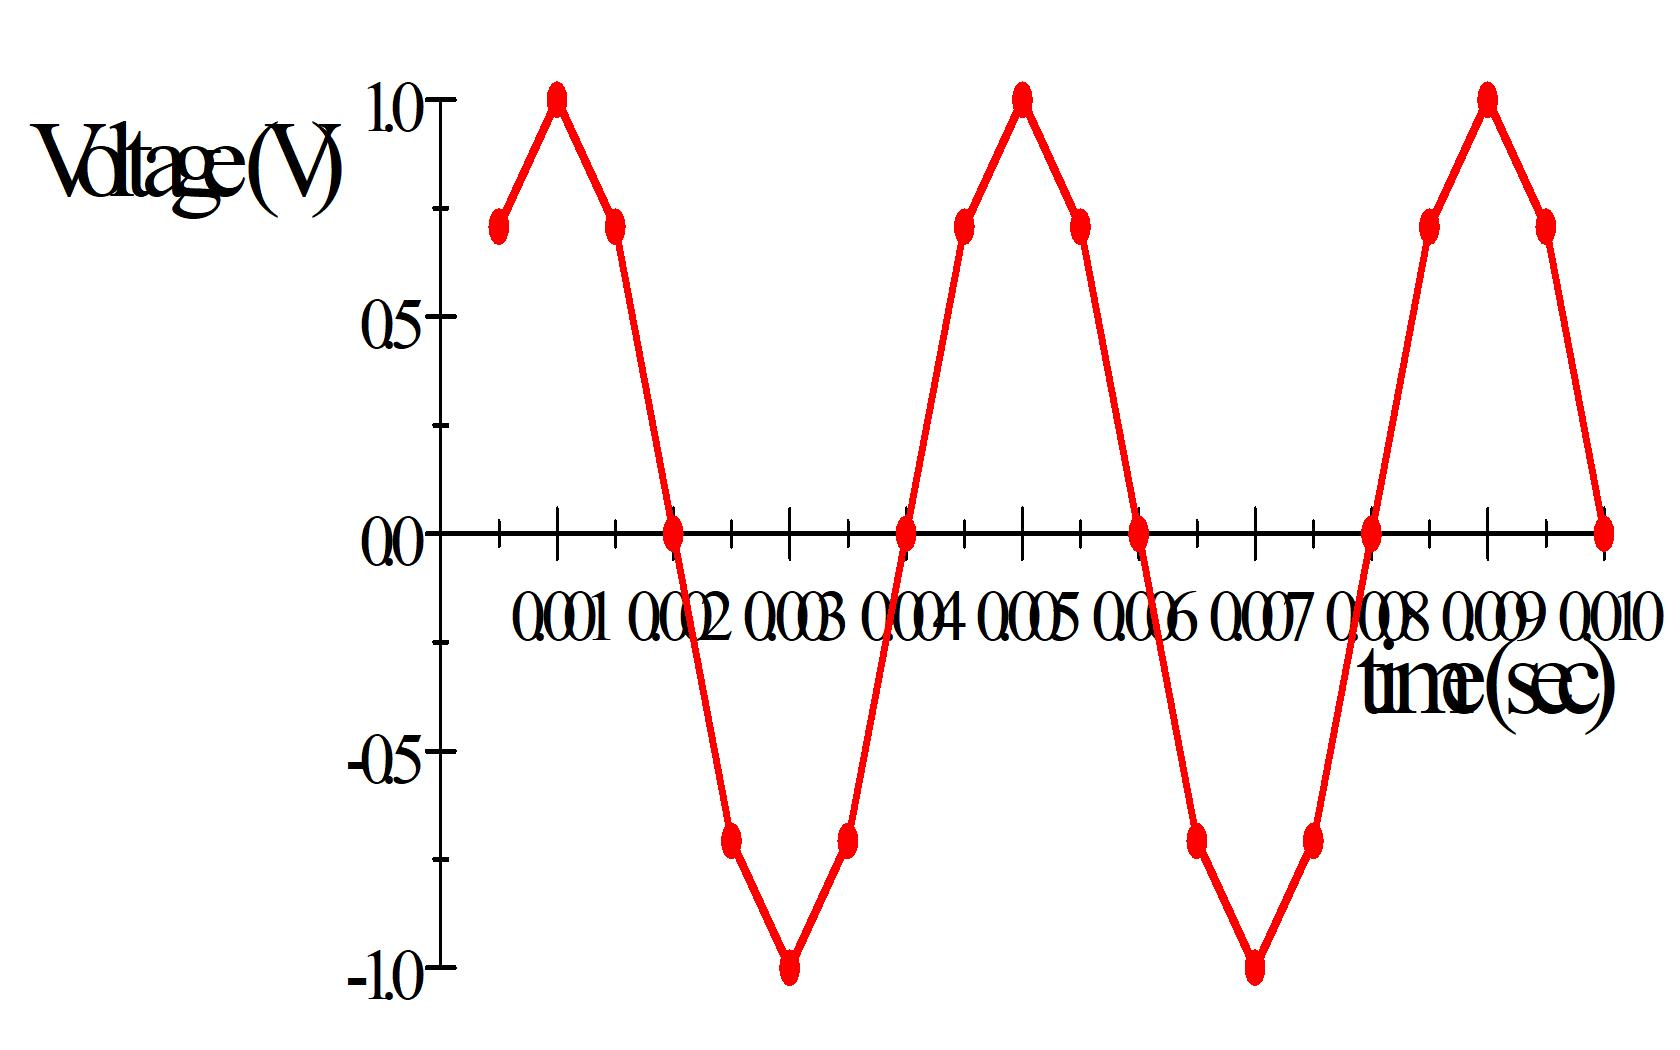
\includegraphics[width=4.4996in,height=1.6354in]{PH4CAX4P}
	\caption{Connecting the measurements from the 250 Hz signal.}
	\label{fig:sine5}
\end{figure}

This problem of having to
take measurements faster than our signal changes is called 
\textbf{aliasing} (because
if you get it wrong, it looks like the wrong function came from the signal
generator). To avoid issues with aliasing, we need to make sure our 
signal frequency is much lower (like
ten times lower) than the frequency at which we can take measurements, 
or we run the risk of being fooled by our measurements.

%In the last lab, we had resonance frequencies that were around $%
%20000\unit{Hz}.$ That is way too high for our Arduinos. We need to change
%capacitors so that our resonance frequency is more like $200\unit{Hz}$, or
%our measurements will be aliased. Suppose we use the following 
%\begin{eqnarray*}
%\mathcal{E} &=&5\unit{V} \\
%L &=&2.3\times 10^{-3}\unit{H} \\
%R &=&10000\unit{%
%%TCIMACRO{\U{3a9}}%
%%BeginExpansion
%\Omega%
%%EndExpansion
%} \\
%f_{resonance} &=&18.552\unit{kHz} \\
%C &=&32\times 10^{-6}\unit{F}
%\end{eqnarray*}
%Our resonance plot will look more like Figure \ref{fig:res2},
%which we could reasonably detect using the Arduino.
%Our measurements might look somewhat ratty, but we should be able to
%see a sine wave and find when it is maximum.
%\begin{figure}[htbp!]
%	\centering
%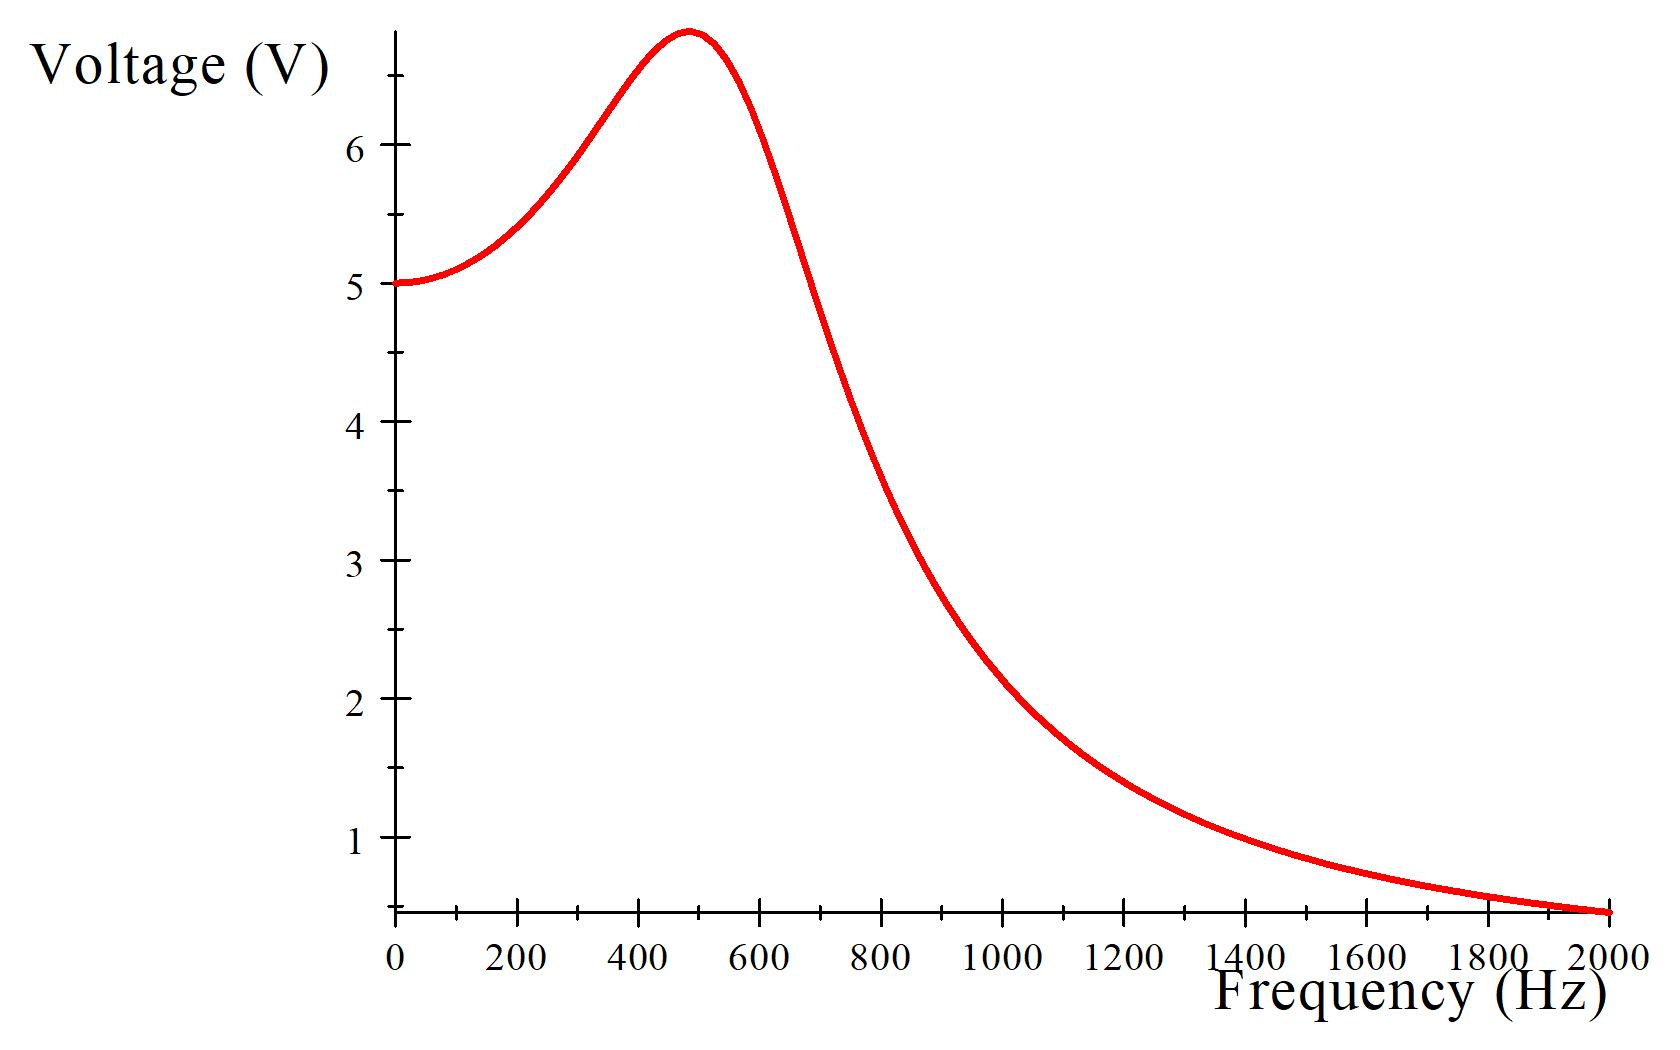
\includegraphics[width=4.4996in,height=3in]{PH4CAX4Q}
%	\caption{Resonance plot for an RLC circuit with a resonant frequency of
%	500 Hz.}
%	\label{fig:res2}
%\end{figure}

\clearpage
\activity
{

\begin{enumerate}
%\item Estimate the inductance of your coil using equation \ref{Solenoid
%Inductance}. You may use your estimate from last week and any insight into
%that estimate that last week's measurements might have given you.
%
%\item Measure the inductance using resonance with an Arduino based
%oscilloscope
%
%\begin{enumerate}
%\item Set up an RLC circuit like we did last lab. Select a capacitor that will
%give you a resonant frequency of a few hundred Hertz.
%Use a signal generators to produce as the source of variable emf. 
%
%\item Build and attach a voltage divider, as diagrammed in Figure 
%\ref{fig:rlc_schematic}. 
%
%\item Test the circuit using an oscilloscope. Again you should see a nice
%sine wave, but now we need to be sure that the voltage is far less than our $%
%5\unit{V}$ limit for our Arduino. We know the voltage is going to be highest
%at resonance. So we need to be careful!
%\begin{center}
%
\includegraphics[width=2.8089in,height=1.4684in]{PH4CAX4S}
%\end{center}
%Once you are satisfied that the voltages will not damage the Arduino, connect
%the output of the voltage divider to the Arduino.
%
%\item Begin collecting voltage data with the Arduino. You can use the serial
%plotter to see your signal. 
%Adjust the frequency of the signal generator until you reach resonance.
%(Note what happens to the amplitude as you tune the dial. This
%should be the same as what you saw on the oscilloscope in the last lab.)
%
%\item Determine your actual resonant frequency, $f_{A}$.
%
%\item Calculate the inductance of your coil based on $f_{A}$. Compare to
%your estimated value. If there is a difference, try to explain it.
%\end{enumerate}
%
%\item Check with your professor to make sure everything is set to start your
%student designed project next week.

\item Obtain a signal generator, and build the circuit in Figure 
	\ref{fig:rlc_schematic}. Attach the two leads of an oscilloscope, and
	tie all of the grounds together.
\item Turn on the signal generator, and set the frequency to 1 Hz. Adjust the
	DC voltage on the power supply, and make sure your oscilloscope 
		displays an image similar to Figure \ref{fig:rlc_osc}. Note
		that the oscilloscope channels will both need to be set to use
		a DC coupling, and you will want to adjust the output amplitude
		of the signal generator so that it puts out a maximum of
		five volts.
\item Load the appropriate code onto the Arduino.
\item Once you are satisfied that the voltages between the two resistors in 
	the voltage divider range only between zero and five volts, connect
		the analog input lead of the Arduino between the resistors, 
		and connect the ground of the Arduino to the other grounds
		in the circuit.
\begin{center}

\includegraphics[width=2.8089in,height=1.4684in]{PH4CAX4S}
\end{center}
\item Using the Serial Plotter in the Arduino IDE, observe the alternating
	voltage read by the Arduino, and verify that your Arduino is 
		``reading'' the signal generator voltages correctly.
\item Begin increasing the frequency of the signal generator, while watching
	the output on the Serial Plotter. At some point, you will notice that
		your output no longer looks like a nice clean sine wave. 
		Record the frequency at which this happens.
\item Investigate even higher frequencies, and observe the aliasing effect on 
	the output of your ``Arudino oscilloscope''.
\end{enumerate}
}
